\documentclass[utf8,english]{gradu3}

\usepackage{graphicx} % for including pictures

\usepackage{amsmath} % useful for math (optional)

\usepackage{booktabs} % good for beautiful tables

\usepackage{csquotes} % ensure proper formatting

\usepackage[authordate,backend=biber,noibid]{biblatex-chicago}

% NOTE: This must be the last \usepackage in the whole document!
\usepackage[bookmarksopen,bookmarksnumbered,linktocpage]{hyperref}

\addbibresource{thesisReferences.bib} % The file name of your bibliography database

\begin{document}

\title{Artificial General Intelligence - a systematic mapping study}
\translatedtitle{Yleistekoäly - systemaattinen kirjallisuuskartoitus}
\studyline{Mathematical Information Technology}
\avainsanat{%
  Pro Gradu,tutkielma, AI, tekoäly}
\keywords{Master's Theses, AGI, AI, artificial intelligence, systematic 
literature mapping, mapping study}
\tiivistelma{%
  
  Tässä suunnitelmassa käydään läpi pro gradu -tutkielman mahdollista aihetta 
  ja tutkimustapaa. TODO: translate when abstract done
}
\abstract{%
  In this thesis, a systematic mapping study is performed on the field of 
  artificial general intelligence. The goal of the study is to gain insight 
  about the recent developments in the study field. This includes the focus 
  points of the current reserch, possible research gaps, and how the research 
  itself is conducted. TODO: more accurate, proper abstract
}

\author{Samu Kumpulainen}
\contactinformation{\texttt{samu.p.kumpulainen@student.jyu.fi}}
% use a separate \author command for each author, if there is more than one
\supervisor{Vagan Terziyan}
% use a separate \supervisor command for each supervisor, if there
% is more than one

\maketitle

\mainmatter

%Remember to use chapters in the thesis itself
\chapter{Introduction}
The thesis will be a systematic research mapping on the field of 
Artificial General Intelligence (AGI). The goal of the thesis is to identify 
the themes and subfields of AGI research in recent years, what is being 
researched recently, and what kind of gaps exist on the field. For a while the 
AGI field was not so active and the more specific approaches, 'narrow AI', 
grew in popularity. Recently, however, the wider, more general artificial 
intelligence has been regaining interest. This kind of mapping study would 
be needed as the research field is complex and there is no clear presentation 
of the current trends and focal points. Creating this king of overview would 
be a valuable asset for future research, as it would enable focusing the 
research on areas less ventured. Furthermore, if an interesting subtopic 
comes up during the process of mapping, more focus may be directed towards 
that in form of more traditional systematic literature review. This option 
is left for further consideration.

What each chapter is about, how the thesis is structured etc.


\chapter{Artificial General Intelligence} 

TODO: Here some chapter introducing text

\section{History of Artificial Intelligence} 
\label{history}

Even though the idea of autonomous machinery has been around since the ancient 
Greek (\cite{}), AI's origins are set around in the 1940s. At the time, 
American science fiction author Isaac Asimov wrote numerous novels and 
short stories about conscious robots and technology's relation to humankind. 
His work has inspired countless people in the field's of AI and computer science
since then (\cite{kaplan2019}).
Also in the 1940s, mathematician Alan Turing's work on Britain's 
code breaking efforts lead to the creation of first electromechanical computer, 
The Bombe (\cite{kaplan2019}). Turing later gave lectures and wrote an article 
titled \emph{"Computing Machinery and Intelligence"} (\cite*{turing1950}), 
in which he presented several ideas later prevalent in AI field, including the
 "Imitation game", a test to measure the intelligence of a machine 
 (\cite{norvig2002}). This later became well known as the Turing test.

The term Artificial Intelligence was coined in 1956 during a two-month workshop 
\emph{Darthmouth Summer Research Project on Artificial Intelligence}, organized 
by John McCarthy and Marvin Minsky (\cite{kaplan2019}). The participants of the 
workshop would later become the most prominent figures of AI research. During 
DSRPAI two researchers, Allen Newell and Herbert Simon presented Logic Theorist,
 their existing reasoning program, capable of proving multiple mathematical 
 theorems (\cite{norvig2002}). Based on this work the two later created General 
 Problem Solver, GPS, which could solve simple puzzles like Towers of Hanoi 
 using human like recursive approach (\cite{newell1959}). The early days of AI 
 research produced many similar results in different areas. IBM's Arthur Samuel 
 created AI programs that learned to play checkers at a strong amateur level 
 (\cite{norvig2002}).
John McCarthy's 1958 paper titled "Programs with common sense", describes Advice 
Taker, a complete but hypothetical AI system with general knowledge about the
world and deductive processes to manipulate it. The paper is still thought to be
relevant today. McCarthy's system was able to acquire new skills in previously
unknown areas without being reprogrammed.

During these years also work on the neural networks started to gain interest.
The initial work of McCulloch and Pitts (\cite*{mcculloch1943}), later
demonstrated by Hebb (\cite{norvig2002}), showed that a neural network is
capable of learning. In 1960s Rosenblatt's work on perceptrons and Widrow and
Hoff's LMS algorithm were some of the biggest advances in the area
(\cite{widrow1995}). The next great discovery that would propel the neural
networks into the focal point of AI research would happen in the mid-1980s when
the backpropagation algorithm originally presented by Bryson and Ho in 1969 was
rediscovered by multiple independent groups (\cite{norvig2002}). Backpropagation
is one of the most widely used algorithms for training neural networks these
days for its relative power and simplicity (\cite{rumelhart1995}).

History of artificial intelligence contains occasional periods of reduced
interest and funding. These so called "AI winters" are a result of high
expectations collapsing under criticism. First period that can be considered an
AI winter started in the 1970s, and Russell and Norvig (\cite*{norvig2002})
present the following possible reasons for it: Firstly, the early programs knew
nothing about their context, and solved the problems via syntactic
manipulations. This was especially apparent on machine translation projects. As
a language cannot be fully understood without knowing the full context of the
sentences and other nuances of the language, accurate translation proved to be a
difficult task. Failed translation efforts lead to funding cuts in the US.
Second difficulty pointed out by (\cite{norvig2002}) was the sheer complexity of
the target problems. As the early AI programs were focused on simple tasks,
finding a solution by trial and error was possible in practice. But as the
problems became more complex, "combinatorial explosion" issue became more
apparent. The issue was also discussed in British scientist James Lighthill's
report on the state of the AI (\cite*{lighthill1973}). The report is considered
to be one of the main reasons why the British government decided to cut all AI
funding in all but two universities. Lastly, the limitations of the data
structures used in AI field, such as perceptrons, restricted the capabilities of
the solutions. According to Russell and Norvig (\cite*{norvig2002}) this lead to
funding cuts also in the neural network research.

During and after the first AI winter, there was a considerable amount of
research relating to expert systems (\cite{norvig2002}). These systems perform
their tasks in a way similar to human experts in the specific, narrow domain,
relying on a knowledge encoded into a set of rules (\cite{myers1986}). This
style of AI research was inspired by the success of DENDRAL
(\cite{buchanan1968}), a system developed at Stanford by Ed Feigenbaum, Bruce
Buchanan and Joshua Lederberg. DENDRAL's purpose was to use data from mass
spectrometer to infer the structure of a given molecule. MYCIN, developed in the
1970s (\cite{shortliffe1975}), incorporated domain knowledge acquired through
expert interviews, with the uncertainty of medical evaluation taken into account
via certainty factors (\cite{norvig2002}).

Expert systems gained commercial interest, leading to increased research and
adoption in the industry. Government investments in Japan lead to increased
funding in United States and Britain, leading to an AI boom in the 1980s
(\cite{norvig2002}). After the boom, at the end of the 1980s, the second AI
winter arrived. Participation in AI conferences dropped, several of the new AI
companies met their end, as did the AI research divisions in larger hardware and
software companies (\cite{nilsson2009}). The imminent burst of the bubble was
foreseen by several leading researchers, but their warnings didn't have
considerable effect (\cite{nilsson2009}).

According to Russell and Norvig (\cite*{norvig2002}), around this time the AI
field started to adopt the scientific method. This means the earlier ways of
proposing completely new theories based on vague evidence or oversimplified
examples have been replaced by basis on existing theories, repeatable
experiments, and real-world examples. This newly discovered open-mindedness then
lead to a complete new ways of looking at the AI research. AI solutions based on
existing theories, such as speech recognition based on hidden Markov models,
enables the researchers to build on the rigorous mathematical theory behind it
(\cite{norvig2002}). Work of Judea Pearl (\cite*{pearl1988}) and Peter Cheeceman
(\cite*{cheeseman1985}) on the probabilistic reasoning lead to it being accepted
back into the AI field. Later Pearl's Bayesian networks have been used to handle
uncertainty in AI problems. They are graphical models that join probabilistic
information and dependencies to events, enabling inference using probabilistic
methods (\cite{goertzel2007}).

%Large datasets? maybe just mention somewhere else if needed

%TODO: Is the history too much? Feels like it could/should be more topic focused, now it might seem a bit overkill...

%TODO: agents ? 

In the 21st century artificial intelligence research has been steadily growing.
According to (\cite{liu2018}), not only has the amount of publications in the
field been increasing, but also the collaboration between researchers. The study
also deduces that that AI has become more open-minded and popular, as the rate
of self-references is reducing. One reason for the rising popularity on the
field is the success that narrow AI solutions have presented in multitude of
problems. For example, in classical game of Go, program called AlphaGo developed
by Google-owned DeepMind, defeated the world champion Lee Sedol in 2015
(\cite{silver2016}). Due to Go's computationally complex nature this was a
impressive feat previously thought impossible. Later DeepMind developed even
more advanced versions of AlphaGo, called AlphaGo Zero, and generalized
AlphaZero, which could even play Shogi and Chess on superhuman level
(\cite{silver2018}).


Recent years majority of the field has been focusing on the narrow AI approaches
(\cite{goertzel2007}). However, the interest in the classical, strong AI has
also been increasing. This can be seen in the publications from many influential
AI researchers. Authors like John McCarthy (\cite*{mccarthy2007}), Nils Nilsson
(\cite*{nilsson2005}) and Marvin Minsky (\cite*{minsky2007}) have voiced their
opinions that efforts to create a more general AI should be pursued. There are
several terms used regarding these efforts. \textbf{Human-level Artificial
Intelligence} (HLAI) aims to reach "human-level intelligence" and common sense,
a goal that according to Marvin Minsky (\cite*{minsky2004}) can be reached by
not using any single method, but a combination of different resources and
methods. Similar term is \textbf{Artificial General Intelligence} (AGI)
presented by Ben Goertzel and Casio Pennachin (\cite*{goertzel2007}). The goal
of AGI is similar to HLAI, to create an AI system that can express general
intelligence instead of being locked into a single domain. On the next chapter
this general approach is presented in more detail, as it is the focus of this
thesis.


\section{Definition}

% Definition of intelligence?
In order to be able to define AGI, or artificial intelligence in general, one
must first consider the definitions of intelligence in general. The exists many
different definitions, in many different branches of science. Legg and Hutter
(\cite*{legg2007}) list over 60 definitions collected from various academic
sources. These include, for example, \emph{"the general mental ability involved
in calculating, reasoning, perceiving relationships and analogies, learning
quickly, storing and retrieving information,using language fluently,
classifying, generalizing, and adjusting to new situations."} (Columbia
Encyclopedia, sixth edition, 2006), \emph{"that facet of mind underlying our
capacity to think, to solve novel problems, to reason and to have knowledge of
the world"} (\cite{anderson2006}), and \emph{"Intelligence is the ability for an
information processing system to adapt to its environment with insufficient
knowledge and resources."} (\cite{wang1995}). Based on the aforementioned
collection of definitions, Legg and Hutter (\cite*{legg2007}) have formed the
following definition: \emph{"Intelligence measures an agent's ability to achieve
goals in a wide range of environments"}. This gives us a single definition which
encompasses the common traits in intelligence definitions. 

%Intelligence is a trait that manifests itself in multitude of ways, making its
%definition but also its measurement a challenge. 

% gardner, piaget, vygotsky
% Measurement? or later when roadmap is discussed?
% in any case, needs something more here, now just quotes :(

Artificial General Intelligence, sometimes referred as "strong ai", according to
Goertzel and Pennachin (\cite*{goertzel2007}) means \emph{"AI systems that
possess a reasonable degree of self-understanding and autonomous self-control,
and have the ability to solve a variety of complex problems in a variety of
contexts, and to learn to solve new problems that they didn't know about at the
time of their creation."}. It can be seen that an agent fulfilling this
definition also possesses the intelligence defined in the previous chapter. In
this thesis terms artificial general intelligence and human-level artificial
intelligence are treated as synonyms, as they pursue more or less the same goal
of general intelligence. Goertzel and Pennachin (\cite*{goertzel2007}) suggest
that the term AGI is more fitting to the area than HLAI as it human-like
approaches are not necessarily used. 

The reason general intelligence is specified instead of plain intelligence is
that there is a need to differentiate it from the domain specific artificial
intelligence, also known as "narrow AI" or "weak AI", that has become prevalent
in AI research in recent past. Terms strong AI and weak AI were coined by John
Searle in 1980 (\cite{searle1980}). Narrow AI means smart solutions that may
learn and improve their performance through training, but they are only focused
on specific type of problems in a specific context. Examples of such AI include
chess engines, autonomous vehicles, and natural language processing. These
solutions may outperform human capabilities, but only in their limited tasks.
When presented a problem outside their domain, they usually perform poorly. As
the above definition by Goertzel and Pennachin describes, AGI is able to
function on different context and tasks without separate human intervention and
reconfiguration.

TODO: check strong ai definition by searle

%TODO: should this roadmap be placed somewhere else? now seems a bit disconnected
As The AGI community is diverse and there are multitude of opinions on the best
approaches and the goals that should be pursued in the research, several
possible roadmaps have been presented in an attempt to create a common basis for
the discussion and research of human-level artificial general intelligence. In
(\cite{adams2012}) a high level roadmap with AGI's initial required capabilities
and scenario-based milestones is suggested, building on previous work and
workshops organized in 2008 and 2009. Presented scenarios can be used to measure
the progress and capabilities of AGI restricting the progress of different
approaches to a single test situation (\cite{adams2012}). More concrete example
is provided by Ben Goertzel and Gino Yu, who outline creation of a AGI-oriented
cognitive architecture based on existing CogPrime architecture
(\cite{goertzel2014map}). A simultaneous development of multiple AGI-style
applications is suggested to maintain the generality of intelligence. CogPrime
is implemented with OpenCog framework, developed by OpenCog Foundation and AI
researcher Ben Goertzel. OpenCog is an attempt to create an open source
framework for artificial general intelligence
(\cite{opencogwiki,goertzel2012cog}).

One motivation behind this thesis is to find out if these roadmaps and their
suggestions have actually had any effect in the direction the AGI research has gone, or have they been ineffective in their attempt. 


\chapter{Systematic literature mapping process}


\label{method}

Systematic literature mapping is a secondary study method that helps to identify
the focal points and research gaps in the subject area, providing an overview of
previous research (\cite{petersen2008}). It is also known as systematic mapping
study or scoping study (\cite{kitchenham2007}). This chapter introduces the
mapping method, describing each phase of the mapping process. The key
differences with a more common study method, systematic literature review (SLR)
are also presented, as well as the reasoning behind this method choice.

\section{Research method description}
\label{method_description}

Systematic mapping is a common research method used in fields such as
evidence-based medicine, but have until recently been rare in software
engineering (\cite{petersen2008}). Kitchenham, Dybå, and Jorgensen
(\cite*{kitchenham2004}) suggested that adopting evidence-based approach to
software engineering research might benefit the industry by ensuring approaches
used are backed by evidence. Aggregating evidence is done by systematic
literature reviews and similar secondary studies, such as mapping studies
(\cite{kitchenham2010}). As researcher bias is one the weak points of secondary
studies, adhering to strict protocol and guidelines is required to minimize it
(\cite{brereton2007}).


The systematic literature mapping in this thesis is following the method
guidelines presented by Petersen et al (\cite*{petersen2008}), later updated in
by Petersen, Vakkalanka and Kuzniarz (\cite*{petersen2015}). The mapping process
overview can be seen in figure~\ref{fig:mapping}. It consists of five separate
phases: \textbf{definition of research questions, conducting search, screening
of papers, keywording, and data extraction and mapping.} Each phase produces a
subresult to be used in the next one. This process results in a systematic map
of the area. This can and should be further visualized using for example bubble
graphs, as it is a powerful way to achieve a quick overview of the field.
(\cite{petersen2008}). This also enables easier recognition of research gaps and
focus points in the target area.


%TODO: SVG picture? now bad quality...
\begin{figure}[h]
  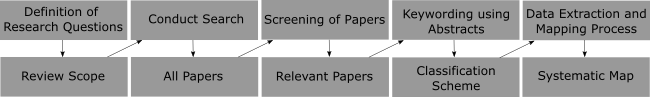
\includegraphics[width=\linewidth]{images/method_graph_L.png}
  \caption{Process model (\cite{petersen2008})}
  \label{fig:mapping}
\end{figure}

% definition of research questions, 
The process begins by defining focused research questions that are aligned with
the goal of the study. The goal of the study often is to create a general
overview of the research area, and to identify the type and quantity of research
(\cite{petersen2008}). Unlike in more focused systematic literature reviews, the
research questions of mapping studies are less focused and cover a broader scope
(\cite{kitchenham2010}). For example, possible research questions on studies
could be: \emph{"Which are the most investigated quality aspects of the software
requirements specifications techniques?"} (\cite{condori2009}) or \emph{"What
efforts have been reported in literature for Software Engineering curriculum
design, implementation, assessment and management?"} (\cite{qadir2011}). These
topic-oriented questions are often combined with research questions regarding
the meta-level information, such as publication year, venue, and research
methods (\cite{petersen2015}).

% conducting search, 
The next phase of the mapping is the initial material search, which can be
conducted multiple ways. Search strings can be formulated from the research
questions, and used on academic databases and search engines
(\cite{petersen2008}). For example, databases such as IEEE Explore and ACM, as
well as aggregators like Google Scholar can be utilized. As the search phrases
should be research question driven, following a criteria such as PICO might
prove to be helpful, as suggested by Kitchenham and Charters
(\cite*{kitchenham2007}). PICO (Population, Intervention, Comparison, Outcomes)
provides an frame to consider research questions' elements and identify
keywords. As the goal is to achieve broad overview of the research, study
outcomes are not taken into account, as this could result in a biased results
(\cite{petersen2008}). The search can also be conducted manually on specific
journals and conference proceedings that cover the target area
(\cite{petersen2008}). This approach is used in this thesis, as it enables
targeting specific reputable and well-known publication venues. TODO: Update
when search method is clear.

% screening of papers, 
After the initial material has been gathered, it is further refined by excluding
papers not relevant to answering the research questions (\cite{petersen2008}).
Separate criteria for both inclusion and exclusion is used to find the papers
fit for further analysis. According to Petersen, Vakkalanka and Kuzniarz
(\cite*{petersen2015}), the criteria may refer to relevance to the topic,
publication venue, time period, language restrictions, and evaluation
requirements. Considering evaluation requirements should be avoided with
systematic maps as it might limit recent trends. Once the criteria is decided,
it is applied to the titles and abstracts of the articles (\cite{petersen2015}).
In case of unclear or poor quality abstracts also the introduction and
conclusion sections of the article may be studied (\cite{petersen2008}). As no
full-text reading is required, screening of papers can be performed rapidly.

% keywording, 
Once the final set of papers is narrowed down and determined, keywording is
performed. As described by Peterson (\cite*{petersen2008}), The keywording
process starts by first by analyzing the research papers' abstracts by searching
possible frequent keywords and prevalent concepts from them. The keywords of
each paper are then combined together to achieve a more general set of concepts.
On some cases having a more detailed inspection of the article might be required
(\cite{petersen2008,petersen2015}). After the final set of keywords is chosen,
they are clustered into categories representing the article population
(\cite{petersen2008}). This emergent classification schema can then be used in
the data extraction phase. 

Different research facets can be used in the classification. For example in
addition to the topical scheme emerging from the keywords, a topic-independent
facet reflecting the research approach can be used. One example of the latter is
the classification of research approaches by Wieringa et. al
(\cite*{wieringa2006}). Wieringa's classification categorizes scientific papers
into six categories such as validation research, solution proposals, and opinion
papers. Using existing topic-independent categorization also enables the
comparison of  different research fields (\cite{petersen2015}).

% data extraction and mapping.
In the final phase of the mapping process, the data extraction is performed by
sorting the papers into the classification schemes present
(\cite{petersen2008}). The schema may evolve during the data extraction process,
changing the categories to match the article population more accurately
(\cite{petersen2015}). The categorization based on the chosen facets results in
a frequency table, i.e. the mapping, with can then be presented with via
visualization and summary statistics. Visualization using for example bubble
plots is preferred, as it is a powerful way to represent the information and map
of the field (\cite{petersen2008}).


\section{Differences with systematic literature reviews}

Because the systematic literature mapping as a study methods is less known in
the field of software engineering, the typical differences between it and more
common secondary study method, systematic literature review, is presented here.
There is many common factors in both of the methods, and as Kitchenham et al.
(\cite{kitchenham2010}) state, \textit{"the distinction between mapping studies
and conventional SLRs can be somewhat fuzzy"}. They also present a view that
mapping studies are just a different type of systematic literature review.

Similar to other secondary study methods, mapping study aims to summarize and
present the research performed in the past. Whereas systematic review focuses on
very narrow research questions, mapping study usually has multiple broader
questions(\cite{kitchenham2010}). Difference in scope breadth can also be seen
in the search strings, as the initial material search for mapping is likely to
return large number of studies (\cite{kitchenham2007, petersen2008}). Mappings
are usually conducted to achieve an overview of the research area, and therefore
the depth of the studies is not as great as in the SLRs. The mapping focuses
more on the thematic analysis of the articles instead of in-depth analysis of
their results or gathering empirical evidence based on their results, which is
often the goal of an traditional SLR (\cite{petersen2008}). Therefore the
quality of the objects of study is not relevant, unless the quality itself is
the aspect to be investigated.

Since both methods have their strengths and weaknesses, using them
complementarily can be an effective combination. As suggested by Petersen et. al
(\cite*{petersen2008}) and Kitchenham et al. (\cite{kitchenham2010}), good
approach is to first get an overview of the research area with systematic map,
and then applying conventional literature review to a specific focus area.
Results of the mapping can provide information on the quantity of available
evidence, which can help targeting the follow-up SLRs more precisely.


\section{Background/reasoning behind method choice}

As a thesis topic, Artificial General Intelligence is a challenging and broad
area. By focusing on the AGI research articles as an object of study, useful
research can still be performed without requiring too much prior knowledge and
expertise on the topic from the author. The reason behind the choice of
systematic literature mapping is that it fits specifically well on creating
overview of the study area. As the research questions of this thesis are broad,
mapping study is a more suitable approach than a conventional SLR.

Due to the complexity of the topic, it can be difficult to enter as a newcomer.
Kitchenham et al. (\cite*{kitchenham2010}) suggest that a systematic mapping of
the field can be useful to researchers new to the area.  It can also be useful
in introducing it to people unfamiliar with the field, both in academia and on
the industry's side. As can be seen from the history of AI research in
\ref{history}, AGI is also a topic that is known of it's fluctuating interest
and popularity, therefore seeing the temporal trends and state of the current
research can be of interest. Mapping study is a good way to achieve that. 

The mapping process guidelines by Petersen et al.
(\cite*{petersen2008,petersen2015}) were chosen to be followed as they were the
most used ones in software engineering community (\cite{petersen2015}). Also the
most popular guideline for systematic literature review by Kitchenham et al.
(\cite*{kitchenham2007}) can be utilized to some degree because of the similarity
of the methods. These guidelines provide clear methodologies for the study. In
addition, the process can further utilize for example the scientific paper
classification scheme presented by Wieringa et al. (\cite{wieringa2006}), as it
provides an useful and straightforward research facet to the categorization
phase of the process. 

\chapter{Conducting the literature mapping}

\textbf{The following text is very raw, will be edited properly later}

In this chapter the systematic literature mapping is conducted. To ensure that
the study is conducted with rigor, documenting it in detail is essential. This
chapter only describes the process, the actual results of the mapping are
presented in chapter \ref{results}. Following the guidelines mentioned in
section \ref{method_description}, the following sections focus on each of the
phases of the study.

TODO: Something more here, mention each subsection?
% search for similar secondary studies?

\section{Research questions}

The following research questions aim to cover the goal of the study, to create an overview of the scientific research performed on the field of AGI. 

\begin{itemize}
  \item[RQ1:] How much, and what kind of research is done in the field of AGI?
  \item[RQ2:] Where and when were the studies published?
  \item[RQ3:] What are the major research topics in the field and have they
  changed over time?
\end{itemize}

The first question focuses on the type and volume of the published AGI related
research. The second question focuses on the publication venue and time of the
articles, showing temporal trends and popular forums for the topic. Research
question three aims to find out the most popular subtopics and their change in the
study's time frame. TODO: how these are answered, does it need to be addressed
here or only later?


\section{conducting search}


- Journal listing and their date ranges etc.

- Why journals were chosen, information about them, reliability, area coverage,
jufo rankings etc.

- search terms here or another section? 

- table showing used search phrases?

High level and/or topical relevance make these the ideal candidates for the review.

Issues are looked only on years \textbf{2015-2019}

\textbf{Sources and databases used}

- \textbf{3 ARTIFICIAL INTELLIGENCE} | citescore 7.7 | Impact factor 6.628.
  Issues 218-277 = 59, articles in issue c. 10,

- \textbf{3 JOURNAL OF ARTIFICIAL INTELLIGENCE RESEARCH} | IF 1.8.
  Issues 52-66 = 14, articles in issue c.20

- \textbf{1 JOURNAL OF ARTIFICIAL GENERAL INTELLIGENCE}.
  Issues = 6, articles in issue c. 2

- \textbf{INTERNATIONAL CONFERENCE ON ARTIFICIAL GENERAL INTELLIGENCE}. Issues =
  5, articles in issue c. 30. This conference seems to be surprisingly active
  and on topic.Not in JUFO rankings.
  
  What about this? Has JUFO ranking. - \textbf{1 EUROPEAN SYMPOSIUM ON
ARTIFICIAL NEURAL NETWORKS, COMPUTATIONAL INTELLIGENCE AND MACHINE LEARNING}.
This would increase article load with 500+ articles, with a low number of
relevant papers. So maybe? Maybe not, as paper amount with IJCAI is already
massive.


  \textbf{==> In total, around 1000 articles concerning AI. Quick sampling shows
  the number actually relevant articles may still be very low.} Should interval
  be lengthened or is this ok?

- \textbf{International joint conference on Artificial Intelligence}
  Massive amount of papers. Manual search not feasible.

  What about performing search on journals? 

Search phrases are used on different databases, limiting the papers to amount
possible to handle

Search can be also done by inspecting relevant journals (like here)

- evaluation of search: test set of known papers, possible here?

\section{Criteria for inclusion, exclusion}
Criteria is presented, and papers are further narrowed down.

All literature accepted for this thesis should be:

\begin{itemize}
  \item presenting and/or relating to Artificial General Intelligence,
  Human-level AI, or similar concept,
  \item written in English,
  \item published between 2015-2019,
  \item a peer-reviewed journal or conference paper, and
  \item available digitally free or as a member of University of Jyväskylä.
\end{itemize}

Piece of literature should be excluded if it is:

\begin{itemize}
  \item a book, a book chapter, or lecture notes (specify!)
  \item TODO?
\end{itemize}

\section{Keywording}
Papers are further analyzed, keywords are extracted from abstracts and text. 

\section{Data extraction and mapping}
keywords are used to create a mapping, working iteratively. Papers are
categorized based on the emergent mapping. What about existing categorizations,
like Kitchenham? Probably should use multiple facets, like kitchenham, and the
emergent schema.

\section{Source material control}
- How the papers were handled
- How graphs etc. were made
- Other meta level information
- Excel, python, etc.

\chapter{Results and analysis}
\label{results}

The results of the thesis will be a clear overview of the recent research in the
field of artificial general intelligence in form of classification data, visual
graphs and further synthesis. As mentioned earlier, if an interesting topic
presents itself during the process of mapping, it may be further examined in a
more focused way, such as literature review. This will be considered at that
time.

\section{Validity threats?}

- performed alone, researcher bias etc (multiple people not possible here),
how rigor is achieved, repeatability, 

Good source on reliability \cite{wohlin2013}

\section{Results of literature mapping}
- Graphs and other visualization, bubble graphs are useful.
- Key topics should be described shortly?

\section{Possible continuation research}

- List of most prominent topics for further research

\chapter{Conclusion}
In this thesis, a systematic literature mapping was conducted on the field of
artificial general intelligence. Results of the study showed that .... 

\printbibliography


\end{document}